\chapter{Vooronderzoek}

	\par In dit hoofdstuk zullen de verschillende resultaten van het vooronderzoek besproken worden. Ook de simulaties in het programma simulink worden kort toegelicht. Op het einde van dit hoofdstuk wordt een compleet systeemoverzicht weergegeven. 

	\section{Quadcopters}

		\subsection{Wat is een quadcopter}
			
			\par Een quadcopter, ook wel quadrocopter genoemd, is een hefschroefvliegtuig dat, zoals de naam al doet vermoeden, aangedreven wordt door vier motoren. In tegenstelling tot een conventionele helikopter maakt een quadcopter gebruik van symmetrisch hellende propellors die in groepen van twee dezelfde draairichting hebben. Op deze manier wordt de tolbeweging die ontstaat door de krachtwerking van de motoren tegengewerkt en gereduceerd tot nul. Dit zorgt ervoor dat de quadcopter tijdens de vlucht niet rondtolt. Bij een klassieke helikopter wordt het opheffen van deze kracht voorzien door de staartrotor.

				\begin{figure}[H]					  
					  \centering
					  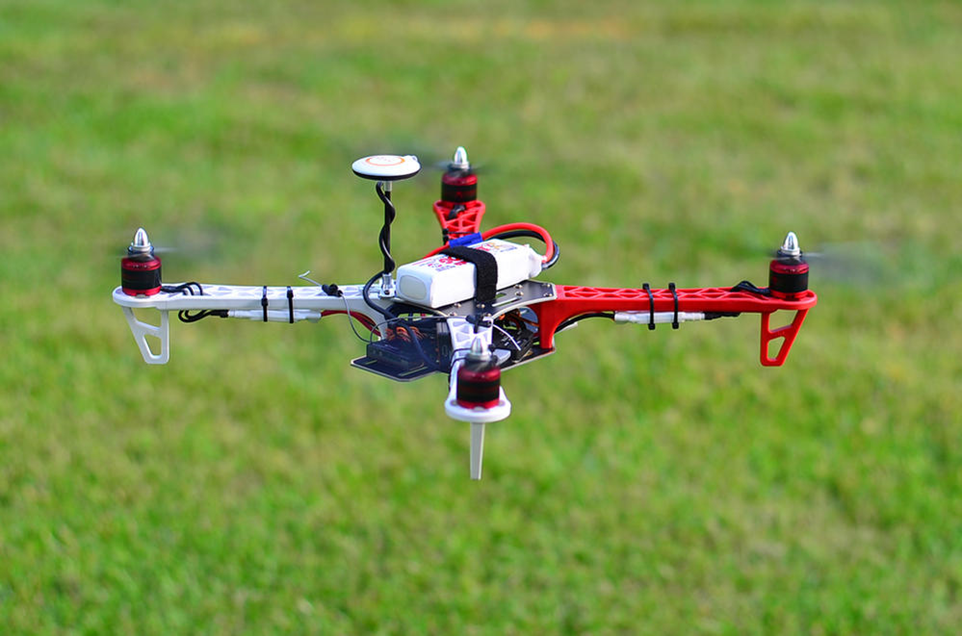
\includegraphics[width=0.5\textwidth]{Vooronderzoek/quad_foto.png}
					  \caption{Quadcopter in actie}
					  \label{quadcopter_foto}
				\end{figure}

			\par Een quadcopter is opgebouwd uit een frame dat vier armen bevat. Op het uiteinde van deze armen zijn de motoren (brushless DC) bevestigd. Om de motoren aan te sturen wordt gebruik gemaakt van een \textquoteleft engine speed controller \textquoteright (ESC). Deze zorgt voor de aansturing van de motoren. Een centrale eenheid regelt zowel de stabilisatie als de invoer van de piloot.

			\par Een quadcopter is van nature onstabiel. Een regelsysteem dat stabilisatie voorziet tijdens de vlucht is nodig. Dit systeem zal ten minste een stabilisatie voorzien rond de roll-, pitch- en yaw-as. Optioneel kan ook een stabilisatie voor drift en hoogte voorzien worden. Deze stabilisatie wordt meestal voorzien door middel van een PID controller voor elke as.

			\par Naast het voorzien van stabilisatie dient er ook gereageerd te worden op de invoer van de piloot. De centrale eenheid (autopilot) implementeert typisch deze functies. Naast het voorzien van deze basisfuncties kunnen nog verschillende opties toegevoegd worden zoals een return-to-home functie, een autoland functie\ldots 

			\par Als basis voor deze autopilot wordt een IMU unit voorzien. Deze beschikt aan de hand van een accelerometer-, magnetometer- en gyroscoop-informatie over de actuele attitude van de quadcopter. Op basis van deze gegevens kan een stabilisatie uitgevoerd worden.

			\par Hiervoor zijn reeds verschillende systemen op de markt. Een populair systeem binnen de amateurpiloten is ArduPilot. Deze autopilot is volledig gebaseerd op Arduino en compatibel met zowat alle quadcopters en kleine vliegtuigen. 

			\par Net zoals ArduPilot zijn zowat alle autopilot systemen momenteel op de markt, gebaseerd op een microcontroller. Het doel van dit projectlab is het onderzoeken of de basisfuncties van een autopilot ook ge\"implementeerd kunnen worden op een FPGA.

		\subsection{Configuraties}

			\par Een quadcopter kan opgebouwd worden op twee verschillende manieren. Afhankelijk van hoe de armen aan het centrale stuk geplaatst worden, verkrijgt men ofwel een \textquoteleft+\textquoteright  ofwel een \textquoteleft x\textquoteright  configuratie. De configuratie wordt dus bepaald door de vliegrichting van de quadcopter ten opzichte van de propellers. In figuur \ref{quad_config} is een overzicht van beide configuraties weergegeven.

				\begin{figure}[H]					  
					  \centering
					  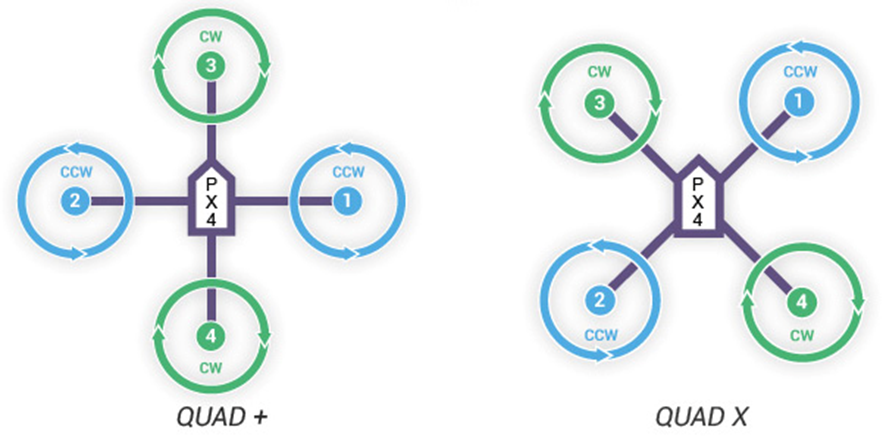
\includegraphics[width=0.65\textwidth]{Vooronderzoek/quad_configuraties.png}
					  \caption{Verschillende configuratiemogelijkheden van een quadcopter}
					  \label{quad_config}
				\end{figure}

			\par De keuze van een bepaalde configuratie heeft een invloed op de manier van besturing, maar ook op het algoritme waarmee de verschillende motoren worden aangestuurd. Wanneer men gebruikt maakt van de  \textquoteleft x\textquoteright configuratie, zijn er twee motoren nodig om een beweging om een bepaalde as uit te voeren. 

			\par Het spreekt voor zich dat het algoritme dat nodig is om de motoren aan te sturen bij een  \textquoteleft x\textquoteright configuratie complexer is dan bij de keuze van een  \textquoteleft +\textquoteright configuratie. Er wordt dus gekozen voor de  \textquoteleft +\textquoteright configuratie binnen dit projectlab.

		\subsection{Besturing van een quadcopter}
			
			\par Om een quadcopter te besturen dienen de motoren op een correcte wijze aangestuurd te worden. Afhankelijk van hoe de motoren aangestuurd worden zal de quadcopter stijgen, dalen, gieren, of stampen. Daarnaast is het ook mogelijk een combinatie van de verschillende bewegingen samen uit te voeren.

			\par Om een quadcopter te laten stijgen of dalen, dienen de vier motoren gelijktijdig versneld of vertraagd te worden. 

			\par Om een quadcopter te laten bewegen om zijn verticale as moet de snelheid van twee motoren die \'e\'enzelfde draairichting hebben verhoogd worden. Hierdoor zal het koppel op de quadcopter toenemen waardoor een gierbeweging zal ontstaan.

			\par Om een quadcopter vooruit, achteruit, link of rechts te laten bewegen in de \textquoteleft + \textquoteright  configuratie volstaat het om \'e\'en motor sneller te laten bewegen dan de anderen. Hierdoor zal de quadcopter kantelen in een bepaalde richting, met een verplaatsing tot gevolg.

			\par In figuren \ref{quad_up_down}, \ref{quad_gieren} en \ref{quad_kantelen} is een overzicht weergegeven van de besturing van een quadcopter in de \textquoteleft + \textquoteright configuratie.

		\begin{figure}[H]
			\centering
				\begin{minipage}[b]{0.3\textwidth}
					\centering
					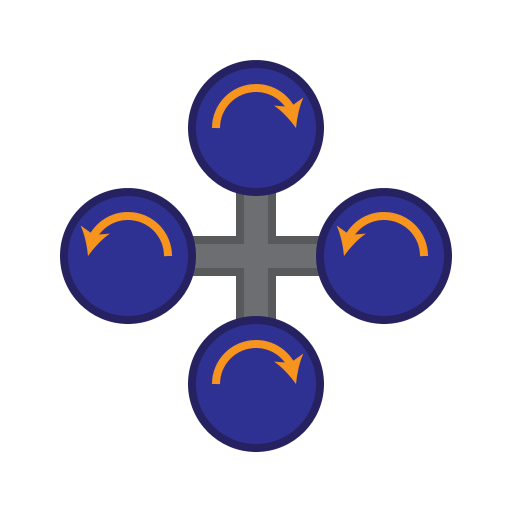
\includegraphics[height = 8cm, valign = b,width=\linewidth]{Vooronderzoek/quad_up_down.png}
					\caption[Omhoog en omlaag]{Omhoog en omlaag}
					\label{quad_up_down}
				\end{minipage}
			\quad
				\begin{minipage}[b]{0.3\textwidth}
					\centering
					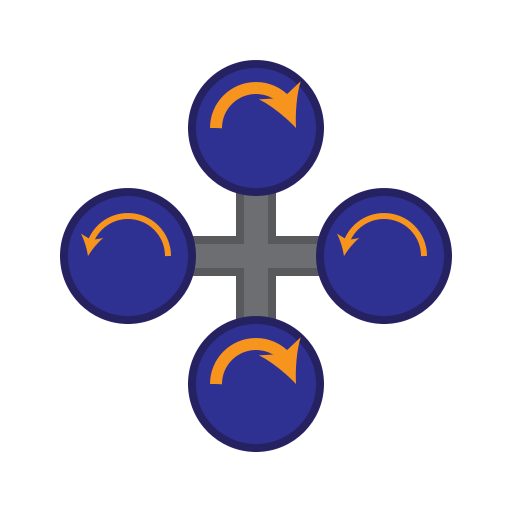
\includegraphics[height = 8cm, valign = b,width=\linewidth]{Vooronderzoek/quad_gieren.png}
					\caption[Gieren]{Gieren \newline \ }
					\label{quad_gieren}
				\end{minipage}
			\quad
				\begin{minipage}[b]{0.3\textwidth}
					\centering
					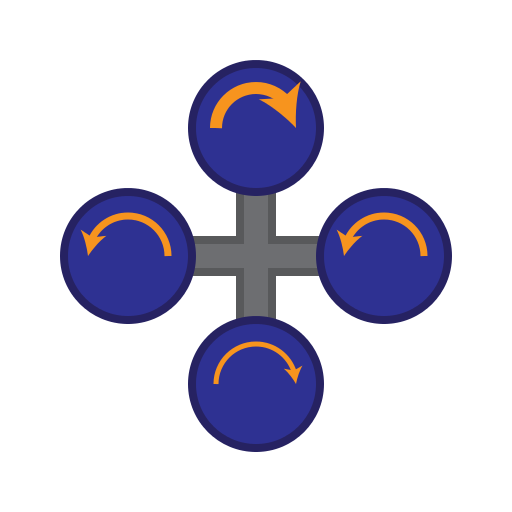
\includegraphics[height = 8cm, valign = b,width=\linewidth]{Vooronderzoek/quad_kantelen.png}
					\caption[Kantelen]{Kantelen \newline \ }
					\label{quad_kantelen}
				\end{minipage}
		\end{figure}

	\section{PID regelaar}

		\par Een PID regelaar is een veel voorkomende regelaar binnen de procesregeling. De afkorting PID staat voor Proportioneel, Integrerend en Differenti\"erend. Dit zijn ook de acties waaruit de regelaar is opgebouwd.

		\subsection{Werkingsprincipe}

			\par De regeling gaat uit van het verschil tussen de gewenste waarde en de actuele gemeten waarde. Dit wordt omschreven als het foutsignaal. Het bijsturen van dit foutsignaal gebeurt in drie parallelle stappen.

				\begin{description}
					
					\item[P-actie:] De proportionele actie zal het foutsignaal versterken met een factor K\textsubscript{p}.

					\item[I-actie:] De integrerende actie zorgt voor een constante sommatie van het foutsignaal. Afhankelijk van hoe lang er een fout is tussen de gemeten en gewenste waarde, zal de integrerende actie meer of minder signaal uitsturen. De K\textsubscript{i} term, ook wel nasteltijd genoemd, bepaald het effect van deze actie. Hoe kleiner deze waarde, hoe krachtiger de actie.

					\item[D-actie:] De differenti\"erende actie zal reageren op de snelheid van verandering van het foutsignaal. Hoe hoger de factor K\textsubscript{d} wordt ingesteld, hoe sneller de wenswaarde bereikt zal worden.

				\end{description}

			\par Wiskundig kan men een PID regelaar als volgt omschrijven:

				\[ u(t) = K_{p}\cdot (e(t)+\frac{\int e(t)dt }{T_{i}}+ T_{d}\cdot \frac{de(t))}{dt}) \]

			\par Hierin is 

				\begin{conditions*}
					U(t)				& De uitgang van de regelaar				\\
					K\textsubscript{p}	& De proportionele actie van de regelaar	\\
					T\textsubscript{i}	& De integratietijd van de regelaar			\\
					T\textsubscript{d}	& De differentiatietijd van de regelaar 	\\
					E(t)				& Het errorsignaal							\\
				\end{conditions*}

			\par Het bepalen van de juiste constanten is een werk van trial-and-error. Dit zal dan ook experimenteel moeten vastgesteld worden op de quadcopter.

		\subsection{Digitalisatie van een PID}

			\par De formule die hierboven weergegeven is, kan als volgt vertaald worden naar een digitaal systeem.

				\[ U\textsubscript{k} = U\textsubscript{k-1} \cdot e\textsubscript{k} + b\textsubscript{0} \cdot + b\textsubscript{1} \cdot e\textsubscript{(k-1)} + b\textsubscript{2} \cdot e\textsubscript{(k-2)} \]

			\par Hierbij is

				\begin{itemize}
					\item[] $ b\textsubscript{0} = K\textsubscript{p}(1+ \frac{T\textsubscript{d}}{T}) $ \\					
					\item[] $ b\textsubscript{1} = K\textsubscript{i}(-1 +  \frac{T}{T\textsubscript{i}} -2\frac{T\textsubscript{d}}{T} ) $ \\		
					\item[] $ b\textsubscript{2} = K\textsubscript{d}(\frac{T\textsubscript{d}}{T}) $ \\
				\end{itemize}

			\par Deze formule kan weergegeven worden in het onderstaande schema.
	
				\begin{figure}[H]					  
					  \centering
					  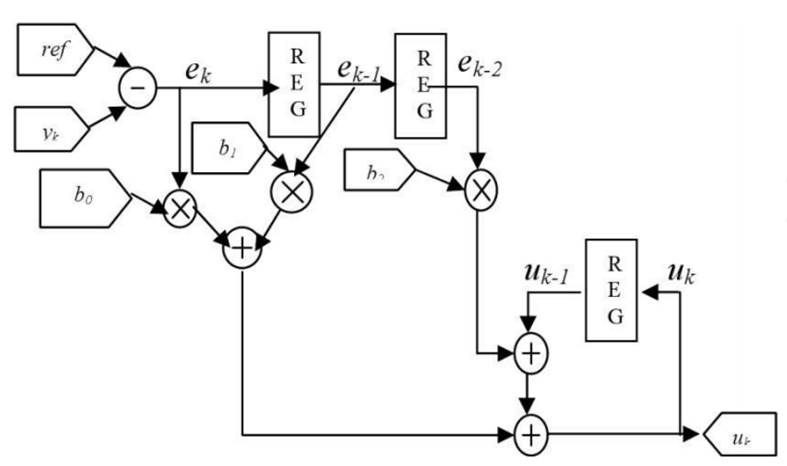
\includegraphics[width=0.8\textwidth]{Vooronderzoek/pid_digitaal_schema.png}
					  \caption{Schematische voorstelling van een PID regelaar}
					  \label{pdi_digitaal_schema}
				\end{figure}

			\par De werking van de in figuur \ref{pdi_digitaal_schema} weergegeven regelaar wordt gevalideerd via het programma Simulink. Op deze manier kan reeds voor de FPGA implementatie gekeken worden of de regelaar zal doen wat er verwacht wordt. Daarnaast vormt deze simulatie een goede basis om het FPGA design te starten. In figuur \ref{pdi_simulink_schema} is de Simulink versie van de PID regelaar weergegeven.

				\begin{figure}[H]					  
					  \centering
					  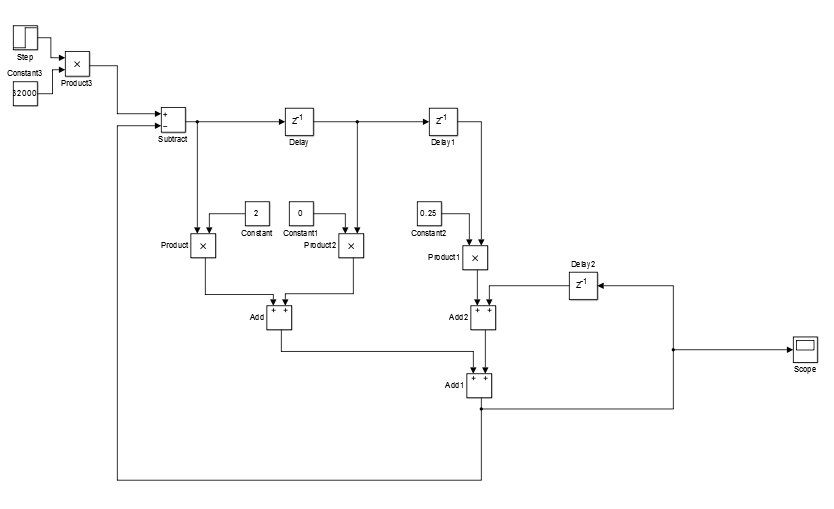
\includegraphics[width=\textwidth]{Vooronderzoek/pid_simulink_simulatie.png}
					  \caption{Simulink voorstelling van een PID regelaar}
					  \label{pdi_simulink_schema}
				\end{figure}

			\par Wanneer men de uitgang aan de ingang koppelt van bovenstaande PID wordt er aangenomen dat de nieuwe gemeten waarde gelijk is aan de uitgang van de PID. Dit levert het volgend resultaat op na simulatie.

				\begin{figure}[H]					  
					  \centering
					  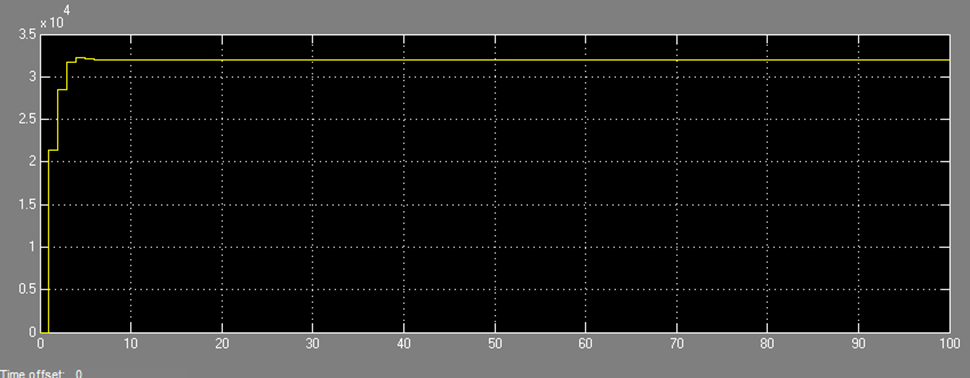
\includegraphics[width=\textwidth]{Vooronderzoek/pid_simulink_resultaat.png}
					  \caption{Resultaat van simulatie PID in Simulink }
					  \label{pdi_simulink_resultaat}
				\end{figure}

			\par In figuur \ref{pdi_simulink_resultaat} is duidelijk de werking van een PID waar te nemen. Het signaal klimt naar de gewenste waarde toe, maakt een kleine overshoot en stabiliseert vervolgens op het gewenste signaal. Dit is ook wat men verwacht van een PID. Men kan dus besluiten dat het schema in figuur \ref{pdi_digitaal_schema} voldoet aan de eisen en ge\"implementeerd kan worden in de FPGA.

	\section{Xilinx DSP48 slices}

		\par De Spartan 6 reeks bevat verschillende DSP48A slices. Deze MAC bouwstenen zijn door Xilinx speciaal ontworpen om DSP toepassingen te realiseren.

			\begin{figure}[H]					  
				  \centering
				  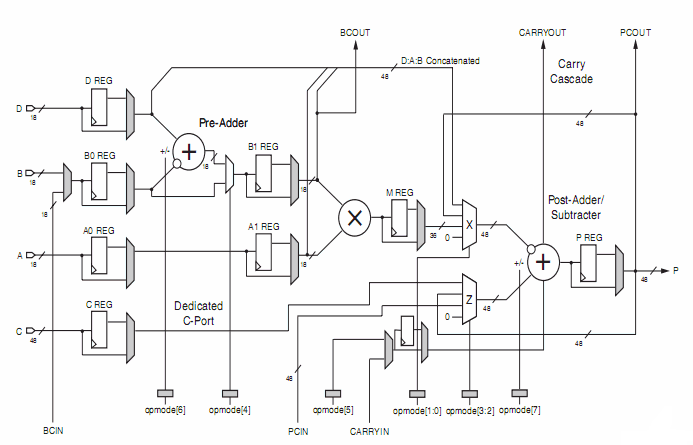
\includegraphics[width=0.90\textwidth]{Vooronderzoek/dsp48a.png}
				  \caption{Interne structuur van een DSP48A slice }
				  \label{pdi_simulink_resultaat}
			\end{figure}

		\par Het doel van een DSP48 slice is het zo performant mogelijk uitvoeren van MAC operaties. Hiervoor zijn verschillende adders en een multiplier binnen het DSP48 slice aanwezig. Als invoer kan een signaal van maximaal 18 bits aangelegd worden. De uitgang is maximaal 48 bit. Hiervan is ook de naam DSP48 afgeleid.

		\par De DSP48A slices kunnen binnen de Xilinx ISE ontwikkelomgeving op verschillende manieren worden ge\"instantieerd. De eenvoudigste methode is via de IP Coregen. De gebruiker maakt stapsgewijs de instellingen op basis van een aantal selecties. Visueel wordt weergegeven welke instellingen gemaakt worden. Een andere manier om een DSP48 Slice te implementeren is door gebruik te maken van een zogenaamde Port Map in de code. Hierbij worden alle instellingen handmatig gemaakt en dient goed rekening gehouden te worden met de datasheet. Een derde manier om DSP48 slices te gebruiken is via de Xilinx System Generator. Dit is een pakket dat in samenwerking met Matlab en Simulink de mogelijkheid voorziet om visueel, door middel van blokken, een systeem samen te stellen en de nodige VHDL code te genereren. 

		\par De Spartan 6SLX9 beschikt over 12 DSP48A slices. Binnen het FPGA zullen deze gebruikt worden waar mogelijk om het gehele proces te versnellen.
\newpage
	\section{Mojo FPGA ontwikkelbord}

		\par Tijdens het projectlab zal gebruik gemaakt worden van het Mojo FPGA ontwikkelbord. Dit bord heeft een Spartan 6 XC6SLX9 FPGA aan boord waarbij de gebruiker beschikt over 84 digitale IO pinnen. Naast de digitale IO pinnen van het Mojo bord zijn er ook 8 analoge inputs voorzien. Deze bevinden zich op een externe ATmega controller die via een SPI interface communiceert met de FPGA.

		\par Het programmeren van het Mojo bord gebeurt op eenvoudige wijze. Via het programma Mojo loader kan een \texttt{.bit} bestand naar de externe ATmega geladen. Telkens wanneer de FPGA opgestart wordt zal het laatst opgeslagen \texttt{.bit} bestand geladen worden op de FPGA. Op deze manier dient na stroomuitval niet steeds opnieuw het \texttt{.bit} bestand geladen te worden.

		\par Er zijn reeds verschillende shields op de markt die het mogelijk maken om het Mojo board verder uit te breiden. Daarnaast is het project volledig open source waardoor er zelf ook makkelijk extra hardware ontwikkeld kan worden. Alle schema\textquotesingle s en PCB layouts zijn via de website van de makers vrij verkrijgbaar.

		\par In afbeelding \ref{mojo} is het Mojo bord weergegeven. Naast de 84 digitale en 8 analoge IO pinnen beschikt het Mojo bord ook over 8 leds die verbonden zijn met de FPGA.

			\begin{figure}[H]					  
				  \centering
				  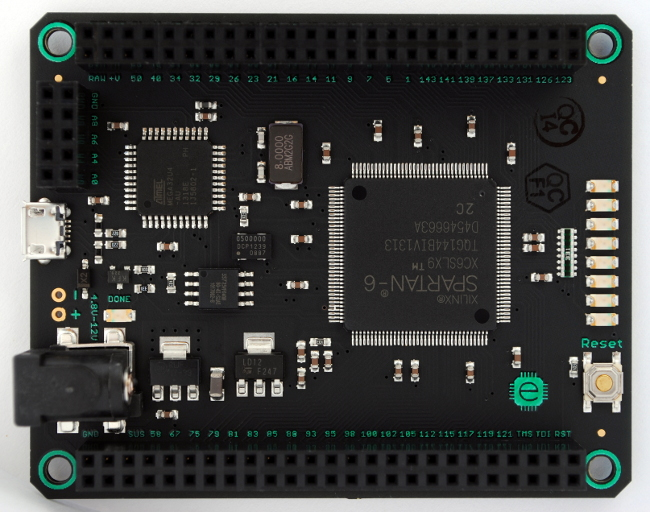
\includegraphics[width=0.6\textwidth]{Vooronderzoek/mojo.png}
				  \caption{Overzicht van het Mojo FPGA ontwikkelbord}
				  \label{mojo}
			\end{figure}
\newpage
	\section{Sensoren}

		\par Om een stabilisatie te voorzien van de quadcopter is het noodzakelijk een inzicht te krijgen van zijn actuele attitude. Hiervoor wordt gebruik gemaakt van een IMU sensor. IMU staat voor inertial measurement unit. Deze unit bevat een combinatie van accelerometers, magnetometers en gyroscopen om zo informatie te verwerven over de huidige attitude van de quadcopter in de ruimte. Om daarbij ook informatie te verschaffen over de hoogte, wordt gebruik gemaakt van de combinatie van een ultrasone sensor en een barometer.

		\subsection{Opmeten van de attitude}

			\subsubsection{Principe}

			\par Een AHRS, attitude and heading reference system, voorziet de gebruiker van informatie over de stand van het vliegtuig. Om dit te berekenen wordt gebruik gemaakt van de data die afkomstig is van een IMU sensor. Zoals reeds hierboven beschreven werd, is een IMU sensor een combinatie van volgende drie sensoren.

				\begin{description}
				
					\item[Accelerometer:] Een accelerometer meet de versnelling van de quadcopter, vaak uitgedrukt in g-krachten. Aan de hand van deze versnelling kan bepaald worden of de quadcopter in een bepaalde richting beweegt of in vrije val is.
				
					\item[Gyroscoop:] Een gyroscoop meet de hoekverdraaiing op, uitgedrukt in radialen per seconde. Zo kan men de draairichting van de quadcopter bepalen. Deze hoekverdraaiing kan op zijn beurt gebruikt worden om de gemeten accelerometerwaarden te corrigeren. Indien de accelerometer namelijk niet in de correcte positie gehouden wordt, is het assenstelsel van de quadcopter verdraaid en zijn de gemeten x, y en z componenten niet correct ten opzichte van het assenstelsel in de re\"ele wereld.

					\item[Magnetometer:] Een magnetometer meet storingen in het aardmagnetisch veld op. Deze data wordt gebruikt om de performatie van de AHRS berekeningen op te voeren.
				
				\end{description}

			\par Aangezien men met de gyroscoop kan opmeten hoe groot de verdraaiing ten opzichte van het originele assenstelsel is, kunnen we het assenstelsel van de accelerometer corrigeren door matrixbewerkingen uit te voeren. Op die manier zijn de gemeten accelerometerwaarden toch te beschouwen vanuit het wereldse assenstelsel.

			\par Uit deze data wordt vervolgens de attitude van de quadcopter berekend. Deze bestaat uit de heading, de pitch-rate en de yaw-rate. 

			\par Vele sensoren gebruiken naast de boven beschreven parameters ook de temperatuur om een kalibratie uit te voeren en de nauwkeurigheid van het systeem te verbeteren.

			\par In figuur \ref{ahrs} is het principe van een AHRS op basis van IMU data weergegeven. 
			
			\begin{figure}[H]					  
				  \centering
				  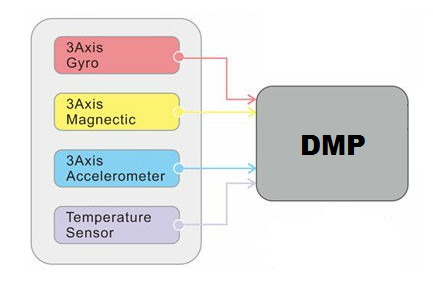
\includegraphics[width=0.6\textwidth]{Vooronderzoek/ahrs.png}
				  \caption{Overzicht van een AHRS systeem}
				  \label{ahrs}
			\end{figure}


			\subsubsection{Sensoren}

				\par Vandaag de dag zijn er verschillende sensoren op de markt te verkrijgen. Onderzoek heeft uitgewezen dat binnen de UAV wereld de MPU reeks van InvenSense vaak gebruikt worden als IMU. Binnen deze reeks van sensoren komen twee sensoren in aanmerking.

					\begin{description}

						\item[MPU 6050:] Deze IMU omvat heel wat mogelijkheden. Zo is er een ingebouwde processor, de DMP (Digital Motion Processor), die reeds heel wat berekeningen op zich kan nemen. Deze DMP is in staat simpele gestures te detecteren, stappen te tellen, filtering uit te voeren van de sensorwaarden en meer aangezien deze volledig naar wens kan ingesteld worden. De nauwkeurigheid van deze IMU is uitstekend, alsook de mogelijkheid tot het herconfigureren van de DMP. De MPU 6050 bevat een 3-assige accelerometer en een 3-assige gyroscoop. Via een I\textsuperscript{2}C is het mogelijk een externe magnetometer aan te sluiten. De data hiervan wordt opgenomen in de DMP bewerkingen.
						
						\item[MPU 9250:] Deze IMU beschikt over exact dezelfde mogelijkheden als de MPU 6050, maar heeft reeds een 3-assige magnetometer aan boord. Er dient dus geen externe magnetometer aangesloten te worden.

					\end{description}

				\par Er werd gekozen om de MPU9250 sensor te gebruiken bij het ontwerp van de quadcopter. Door de interne filter binnen de DMP wordt een Kalman filter overbodig in het FPGA ontwerp.

		\section{Serial peripheral interface}

			\par SPI is een veelgebruikt protocol voor communicatie tussen twee apparaten. Een SPI-bus bestaat uit vier signalen.

				\begin{description}

					\item[MOSI:] (Master Out Slave In) Dit signaal is de uitgang van de master en vormt de ingang van het slave apparaat. Via dit kanaal wordt informatie van de master naar de slave verstuurd.

					\item[MISO:] (Master In Slave Out) Dit signaal is de uitgang van de slave en vormt de ingang van het master apparaat. Via dit kanaal wordt informatie van de slave naar de master verstuurd.

					\item[SCLK:] (Serial Clock Line) Dit kanaal wordt gebruikt als klok. Het is het master apparaat dat de klok voorziet voor het slave apparaat. Data wordt enkel verstuurd en ontvangen als er een kloksignaal is.

					\item[SS:] (Slave Select) Via een slave select kan de master kiezen uit verschillende slave apparaten waarmee hij wil communiceren. Op deze manier kan een communicatie opgezet worden met meerdere apparaten door middel van \'e\'en master apparaat.

				\end{description}

			\par Zoals reeds eerder werd aangehaald, bestaat een SPI interface uit \'e\'en master apparaat en verschillende slave apparaten. Hierbij kan de master communiceren met elke slave, maar een slave kan enkel communiceren met de master. Aan de hand van een uniek slave select signaal voor elke slave wordt de selectie gemaakt. De communicatie gebeurt full duplex. 

			\par De vereiste voor de klok is dat zijn frequentie lager moet zijn dan de maximale frequentie van de betrokken toestellen. Binnen SPI zijn er twee parameters waarbij rekening gehouden moet worden.


				\begin{description}

					\item[CPOL:] De Clock polarity geeft aan wat de standaard waarde is van het kloksignaal wanneer de SPI-bus zich in de idle toestand bevindt. 

					\item[CPHA:] De Clock phase geeft aan op welke edge van het signaal gesampled zal worden. Een 0 geeft aan dat er op de rising edge gesampled wordt. Een 1 geeft aan dat er op de falling edge gesampled wordt.

				\end{description}

			\par Door het combineren van bovenstaande parameters kan men vier verschillende modi onderscheiden binnen de SPI interface. In figuur \ref{spi_clock} is een overzicht weergegeven van een SPI communicatie tussen twee apparaten. Hierbij zijn de CPOL en CPHA beide ingesteld op 0.

				\begin{figure}[H]					  
					  \centering
					  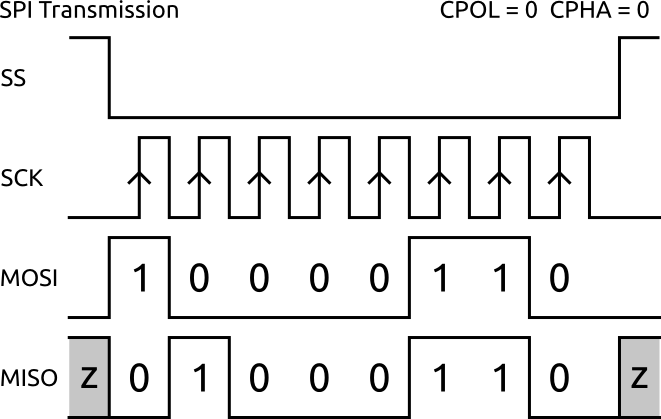
\includegraphics[width=0.6\textwidth]{Vooronderzoek/spi.png}
					  \caption{Overzicht van SPI communicatie tussen master en slave}
					  \label{spi_clock}
				\end{figure}

			\par Op het moment dat de master een clock genereert, zal de communicatie aanvatten. Zowel de master als de slave zullen gelijktijdig data uitwisselen.  

			\par Wanneer de SS naar een lage toestand gebracht wordt, zal de slave geselecteerd worden. Vervolgens genereert de master het kloksignaal en start daarbij ook met versturen van data. Het slave apparaat zal ook starten met sturen van data op de wijzigende flanken van de klok. Wanneer de communciatie voltooid is, stopt de klok en wordt de SS weer naar hoge toestand gebracht.

			\par Om data van de slave op te vragen, moet dus eerst een bericht verzonden worden van welke data men wil opvragen. Daarna moet men nog een bericht versturen om de data te ontvangen. Dit is nodig aangezien het zenden en ontvangen steeds gelijktijdig gebeurt.
\newpage
		\section{Systeemoverzicht}

			\par De resultaten van dit vooronderzoek hebben geleid tot een systeem dat in staat is om de attitude van de quadcopter te controleren. Dit systeem dient in de volgende fase van het project ge\"implementeerd te worden in een FPGA. In figuur \ref{systeemoverzicht} is een overzicht van dit systeem weergegeven.

				\begin{figure}[H]					  
					  \centering
					  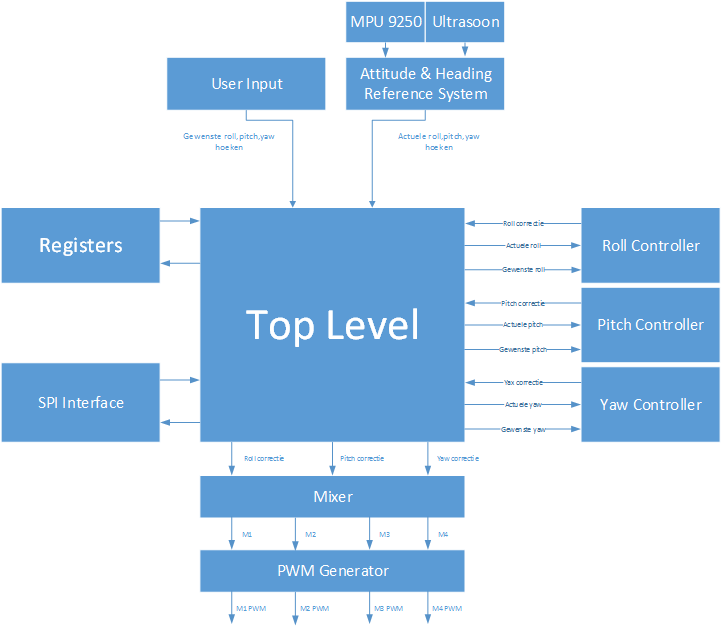
\includegraphics[width=\textwidth]{Vooronderzoek/blokschema.png}
					  \caption{Schematische voorstelling van de quadcopter autopilot}
					  \label{systeemoverzicht}
				\end{figure}
\newpage
			\par In de figuur kan men volgende blokken onderscheiden.

				\begin{description}

					\item[User input:] Deze blok is verantwoordelijk voor het afhandelen van de gebruikersinvoer. Deze is afkomstig van de RF antenne. Een PWM signaal per kanaal dient gelezen te worden. Dit PWM signaal wordt door het toplevel doorgegeven aan de PID controllers om zo de gewenste actie te ondernemen.

					\item[Registers:] In de registers worden alle verschillende instellingen bewaard. Naast deze instellingen worden ook waarden aangeboden aan de gebruiker. Via een SPI interface kan het register gelezen en beschreven worden.

					\item[SPI interface:] De SPI slave interface maakt het mogelijk om zowel te communiceren met een externe microcontroller als de MPU9250 die dienst doet als IMU uit te lezen.

					\item[Mixer:] De mixer is verantwoordelijk voor de verwerking van alle data die afkomstig is van de PID controllers voor rol, pitch en yaw. Aan de hand van deze informatie zal de mixer de geschikte PWM waarden berekenen voor de motoren. Hierbij zal rekening gehouden worden met de maxima en minima die ingesteld zijn in de registers.

					\item[PWM generator:]  De BLDC motoren worden aangestuurd door middel van een PWM signaal. De PWM generator zal voor elke motor een geschikt PWM signaal genereren op basis van de uitvoer van de mixer.

					\item[Roll controller:] De roll-controller stabiliseert het rollkanaal van de quadcopter. Naast de gebruikersinvoer vormt ook de roll-info van het AHRS een input voor deze controller.

					\item[Pitch controller:] De pitch-controller stabiliseert het pitchkanaal van de quadcopter. Naast de gebruikersinvoer vormt ook de pitch-info van het AHRS een input voor deze controller.

					\item[Yaw controller:]De yaw-controller stabiliseert het yawkanaal van de quadcopter. Naast de gebruikersinvoer vormt ook de yaw-info van het AHRS een input voor deze controller.

					\item[Attitude \& heading reference system:] Het AHRS geeft meer informatie over de attitude en heading van de quadcopter. Hiervoor gebruikt dit systeem verschillende sensoren. Dit AHRS systeem zal uitgevoerd worden op een aparte microcontroller en via een SPI interface waarden doorgeven aan het autopilot systeem.

				\end{description}

			\par In het volgende hoofdstuk zullen alle stappen besproken worden die nodig zijn om bovenstaande blokken te implementeren.